\documentclass[11pt,a4paper]{article}

% ============================================================================
% PACKAGES
% ============================================================================
\usepackage[utf8]{inputenc}
\usepackage[T1]{fontenc}
\usepackage{helvet}
\renewcommand{\familydefault}{\sfdefault}
\usepackage[margin=2.2cm, headheight=25pt]{geometry}
\usepackage{xcolor}
\usepackage{colortbl}
\usepackage{booktabs}
\usepackage{tabularx}
\usepackage{array}
\usepackage{graphicx}
\usepackage{tikz}
\usepackage{fancyhdr}
\usepackage{enumitem}
\usepackage{multirow}
\usepackage{calc}
\usepackage{amssymb}
\usepackage{pifont}
\usetikzlibrary{shapes.geometric, arrows, positioning, calc, patterns}

% ============================================================================
% COLOR DEFINITIONS
% ============================================================================
\definecolor{miloprimary}{RGB}{37, 99, 235}
\definecolor{milosecondary}{RGB}{99, 102, 241}
\definecolor{miloaccent}{RGB}{14, 165, 233}
\definecolor{freegray}{RGB}{107, 114, 128}
\definecolor{bronzecolor}{RGB}{205, 127, 50}
\definecolor{silvercolor}{RGB}{156, 163, 175}
\definecolor{goldcolor}{RGB}{234, 179, 8}
\definecolor{platinumcolor}{RGB}{100, 116, 139}
\definecolor{successgreen}{RGB}{34, 197, 94}
\definecolor{warningorange}{RGB}{249, 115, 22}
\definecolor{dangerred}{RGB}{239, 68, 68}
\definecolor{lightbg}{RGB}{248, 250, 252}
\definecolor{darktext}{RGB}{30, 41, 59}
\definecolor{infoblue}{RGB}{59, 130, 246}
\definecolor{darkgreen}{RGB}{22, 163, 74}

% ============================================================================
% HEADER/FOOTER CONFIGURATION
% ============================================================================
\pagestyle{fancy}
\fancyhf{}
\fancyhead[L]{\textcolor{miloprimary}{\textbf{MILO APP}}}
\fancyhead[R]{\textcolor{freegray}{Cost Analysis v3.1}}
\fancyfoot[C]{\textcolor{freegray}{\thepage}}
\renewcommand{\headrulewidth}{2pt}
\renewcommand{\headrule}{\hbox to\headwidth{\color{miloprimary}\leaders\hrule height \headrulewidth\hfill}}

% ============================================================================
% CUSTOM COMMANDS
% ============================================================================
\newcommand{\alertbox}[3]{%
    \begin{tikzpicture}
        \node[fill=#1!12, draw=#1, line width=2pt, rounded corners=8pt,
              inner sep=15pt, text width=\textwidth-35pt, align=left] {
            \textcolor{#1}{\textbf{\large #2}}\\[8pt]
            #3
        };
    \end{tikzpicture}%
}

\newcommand{\statbox}[3]{%
    \begin{tikzpicture}
        \node[fill=#1!10, draw=#1, line width=1.5pt, rounded corners=6pt,
              minimum width=3.6cm, minimum height=2cm, align=center] {
            \textcolor{#1}{\textbf{\small #2}}\\[5pt]
            \textcolor{darktext}{\textbf{\Large #3}}
        };
    \end{tikzpicture}%
}

\newcommand{\cmark}{\textcolor{successgreen}{\ding{51}}}
\newcommand{\xmark}{\textcolor{dangerred}{\ding{55}}}
\newcommand{\wmark}{\textcolor{warningorange}{\ding{115}}}

% ============================================================================
% DOCUMENT BEGIN
% ============================================================================
\begin{document}

% ============================================================================
% TITLE PAGE
% ============================================================================
\begin{center}
    \vspace*{0.3cm}
    {\Huge\textcolor{miloprimary}{\textbf{MILO APP}}}\\[0.4cm]
    {\LARGE\textcolor{milosecondary}{Comprehensive Cost Analysis v3.1}}\\[0.2cm]
    {\large\textcolor{freegray}{Research-Based Pricing with Sustainable Unit Economics}}\\[0.7cm]

    
\begin{tikzpicture}
        \node[fill=miloprimary!10, draw=miloprimary, line width=1.5pt, rounded corners=8pt,
              inner sep=12pt] {
            \textcolor{miloprimary}{\textbf{DeepmAInd B.V.} \quad|\quad Version 3.1 \quad|\quad January 2026}
        };
    \end{tikzpicture}
\end{center}

\vspace{0.5cm}

% ============================================================================
% MARKET RESEARCH FOUNDATION
% ============================================================================
\section*{\textcolor{miloprimary}{Market Research Foundation}}

\begin{center}
\alertbox{infoblue}{Consumer Transaction Data (Federal Reserve, 2024)}{
According to the \textbf{Federal Reserve's Diary of Consumer Payment Choice}, U.S. consumers made an average of \textbf{48 payments per month} in 2024---the highest recorded. Of these:
\begin{itemize}[leftmargin=1.5em, itemsep=3pt]
    \item \textbf{77\%} are in-person transactions (generating physical/digital receipts)
    \item \textbf{23\%} are remote/online purchases
    \item Average in-person receipt-generating transactions: \textbf{35--40 per month}
\end{itemize}
\vspace{4pt}
This research forms the basis for our tier volume design, ensuring tiers align with actual consumer behavior patterns across all retail categories (groceries, dining, gas, retail, pharmacy, services, etc.).
}
\end{center}

\vspace{0.5cm}

% ============================================================================
% EXECUTIVE SUMMARY
% ============================================================================
\section*{\textcolor{miloprimary}{Executive Summary}}

\begin{center}
\renewcommand{\arraystretch}{1.6}
\begin{tabular}{>{\raggedright\arraybackslash}p{5.5cm} >{\centering\arraybackslash}p{2.5cm} >{\centering\arraybackslash}p{2.5cm} >{\centering\arraybackslash}p{2.5cm}}
\toprule
\rowcolor{miloprimary!15}
\textbf{Metric} & \textbf{Year 1} & \textbf{Year 2} & \textbf{Year 3} \\
\midrule
\textbf{Total Revenue} & \$144K & \$720K & \$1.8M \\
\rowcolor{lightbg}
\textbf{Total Variable Costs} & \$36K & \$116K & \$232K \\
\textbf{Total Fixed Costs} & \$260K & \$510K & \$755K \\
\rowcolor{lightbg}
\textbf{Total Operating Costs} & \$296K & \$626K & \$987K \\
\textbf{Operating Profit/(Loss)} & (\$152K) & \$94K & \$813K \\
\rowcolor{successgreen!15}
\textbf{Operating Margin} & -106\% & \textbf{13\%} & \textbf{45\%} \\
\bottomrule
\end{tabular}
\end{center}

\vspace{0.5cm}

% Key Metrics Summary
\begin{center}
    \statbox{successgreen}{All Tiers Positive}{Gross Margin}
    \hspace{0.3cm}
    \statbox{miloprimary}{Avg. Margin}{19\%}
    \hspace{0.3cm}
    \statbox{darkgreen}{Break-even}{Year 2}
    \hspace{0.3cm}
    \statbox{goldcolor}{Year 3 Profit}{\$813K}
\end{center}

\vspace{0.5cm}

\begin{center}
\alertbox{successgreen}{Sustainable Unit Economics Achieved}{
The v3.1 pricing structure ensures \textbf{positive gross margins on all paid tiers} (18--19\%), with a simplified 4-tier model (Bronze, Silver, Gold, Platinum). Tier volumes are aligned with actual consumer transaction patterns (35--40 receipts/month average), creating realistic value propositions for each user segment.
}
\end{center}

\newpage

% ============================================================================
% PRICING STRUCTURE
% ============================================================================
\section*{\textcolor{miloprimary}{Pricing Structure v3.1}}

\subsection*{\textcolor{milosecondary}{Research-Based Tier Design}}

\begin{center}
\renewcommand{\arraystretch}{1.6}
\begin{tabular}{>{\centering\arraybackslash}p{2.8cm} >{\centering\arraybackslash}p{2.2cm} >{\centering\arraybackslash}p{2.2cm} >{\centering\arraybackslash}p{2.2cm} >{\centering\arraybackslash}p{2.8cm} >{\centering\arraybackslash}p{2.2cm}}
\toprule
\rowcolor{miloprimary!15}
\textbf{Tier} & \textbf{Receipts/Mo} & \textbf{Monthly} & \textbf{Annual} & \textbf{Target User} & \textbf{Features} \\
\midrule
\rowcolor{freegray!8}
\textcolor{freegray}{\textbf{Free Trial}} & 15 & Free & -- & New users & \cellcolor{successgreen!15}\textcolor{successgreen}{\textbf{Full}} \\
\rowcolor{bronzecolor!10}
\textcolor{bronzecolor}{\textbf{Bronze}} & 20 & \$2 & \$20 & Light trackers & \cellcolor{successgreen!15}\textcolor{successgreen}{\textbf{Full}} \\
\rowcolor{silvercolor!10}
\textcolor{silvercolor}{\textbf{Silver}} & 40 & \$4 & \$40 & Average users & \cellcolor{successgreen!15}\textcolor{successgreen}{\textbf{Full}} \\
\rowcolor{goldcolor!10}
\textcolor{goldcolor}{\textbf{Gold}} & 60 & \$6 & \$60 & Active trackers & \cellcolor{successgreen!15}\textcolor{successgreen}{\textbf{Full}} \\
\rowcolor{platinumcolor!10}
\textcolor{platinumcolor}{\textbf{Platinum}} & 100 & \$10 & \$100 & Households & \cellcolor{successgreen!15}\textcolor{successgreen}{\textbf{Full}} \\
\bottomrule
\end{tabular}
\end{center}

\vspace{0.5cm}

\subsection*{\textcolor{milosecondary}{Tier Rationale Based on Transaction Research}}

\begin{center}
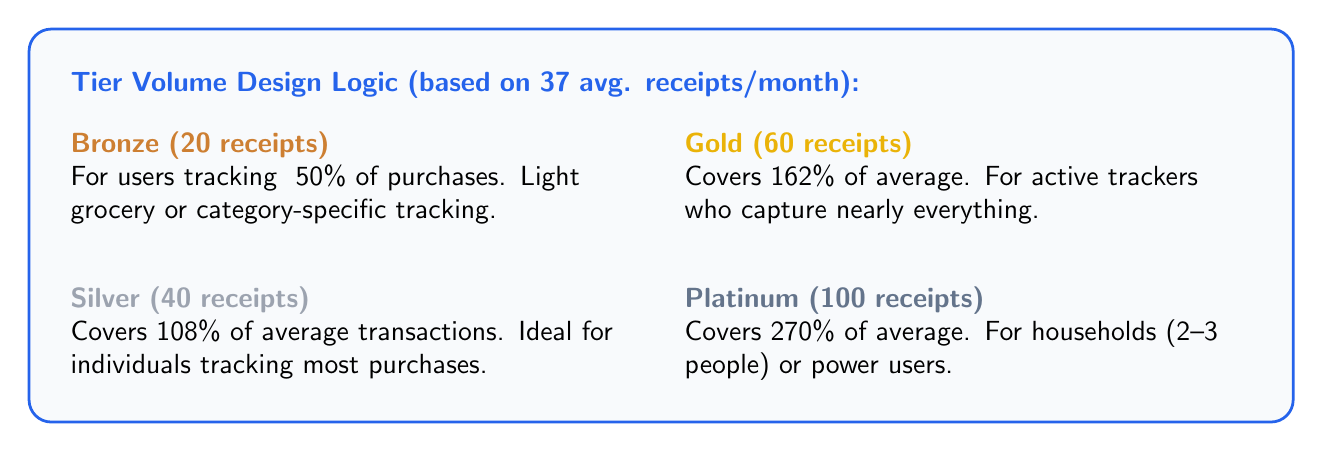
\begin{tikzpicture}
    \node[fill=lightbg, draw=miloprimary, line width=1pt, rounded corners=8pt,
          inner sep=15pt, text width=15cm, align=left] {
        \textbf{\textcolor{miloprimary}{Tier Volume Design Logic (based on 37 avg. receipts/month):}}\\[10pt]
        \begin{minipage}[t]{0.48\textwidth}
            \textcolor{bronzecolor}{\textbf{Bronze (20 receipts)}}\\
            For users tracking ~50\% of purchases. Light grocery or category-specific tracking.\\[8pt]

            \textcolor{silvercolor}{\textbf{Silver (40 receipts)}}\\
            Covers 108\% of average transactions. Ideal for individuals tracking most purchases.
        \end{minipage}
        \hfill
        \begin{minipage}[t]{0.48\textwidth}
            \textcolor{goldcolor}{\textbf{Gold (60 receipts)}}\\
            Covers 162\% of average. For active trackers who capture nearly everything.\\[8pt]

            \textcolor{platinumcolor}{\textbf{Platinum (100 receipts)}}\\
            Covers 270\% of average. For households (2--3 people) or power users.
        \end{minipage}
    };
\end{tikzpicture}
\end{center}

\vspace{0.5cm}

\begin{center}

\begin{tikzpicture}
    \node[fill=successgreen!10, draw=successgreen, line width=1pt, rounded corners=5pt,
          inner sep=10pt, text width=14cm, align=center] {
        \textcolor{darkgreen}{\textbf{Annual Savings:}} All annual plans offer \textbf{17\% discount} compared to monthly billing
    };
\end{tikzpicture}
\end{center}

\newpage

% ============================================================================
% VARIABLE COSTS ANALYSIS
% ============================================================================
\section*{\textcolor{miloprimary}{Variable Costs Analysis}}

\subsection*{\textcolor{milosecondary}{Per-User Variable Cost by Tier}}

\begin{center}
\renewcommand{\arraystretch}{1.6}
\begin{tabular}{>{\raggedright\arraybackslash}p{3.5cm} >{\centering\arraybackslash}p{2cm} >{\centering\arraybackslash}p{2cm} >{\centering\arraybackslash}p{2cm} >{\centering\arraybackslash}p{2cm} >{\centering\arraybackslash}p{2cm}}
\toprule
\rowcolor{miloprimary!15}
\textbf{Component} & \textbf{Trial} & \textbf{Bronze} & \textbf{Silver} & \textbf{Gold} & \textbf{Platinum} \\
\midrule
\textbf{Receipt Limit} & 15 & 20 & 40 & 60 & 100 \\
\rowcolor{lightbg}
\textbf{Veryfi OCR (\$0.08)} & \$1.20 & \$1.60 & \$3.20 & \$4.80 & \$8.00 \\
\textbf{Gemini API} & \$0.01 & \$0.02 & \$0.03 & \$0.05 & \$0.08 \\
\rowcolor{lightbg}
\textbf{Firebase Storage} & \$0.01 & \$0.01 & \$0.01 & \$0.02 & \$0.02 \\
\midrule
\rowcolor{warningorange!10}
\textbf{Total Variable Cost} & \textbf{\$1.22} & \textbf{\$1.63} & \textbf{\$3.24} & \textbf{\$4.87} & \textbf{\$8.10} \\
\bottomrule
\end{tabular}
\end{center}

\vspace{0.5cm}

\subsection*{\textcolor{milosecondary}{Gross Margin Analysis by Tier}}

\begin{center}
\renewcommand{\arraystretch}{1.6}
\begin{tabular}{>{\raggedright\arraybackslash}p{2.8cm} >{\centering\arraybackslash}p{1.8cm} >{\centering\arraybackslash}p{2.2cm} >{\centering\arraybackslash}p{2.2cm} >{\centering\arraybackslash}p{2.2cm} >{\centering\arraybackslash}p{2.5cm}}
\toprule
\rowcolor{miloprimary!15}
\textbf{Tier} & \textbf{Price} & \textbf{Variable Cost} & \textbf{Gross Profit} & \textbf{Gross Margin} & \textbf{Status} \\
\midrule
\rowcolor{freegray!8}
\textcolor{freegray}{\textbf{Free Trial}} & \$0.00 & \$1.22 & -\$1.22 & -100\% & \cellcolor{freegray!15}\textcolor{freegray}{CAC Investment} \\
\rowcolor{bronzecolor!10}
\textcolor{bronzecolor}{\textbf{Bronze}} & \$2.00 & \$1.63 & \$0.37 & \textbf{18.5\%} & \cellcolor{successgreen!20}\textcolor{darkgreen}{\textbf{Healthy}} \\
\rowcolor{silvercolor!10}
\textcolor{silvercolor}{\textbf{Silver}} & \$4.00 & \$3.24 & \$0.76 & \textbf{19.0\%} & \cellcolor{successgreen!20}\textcolor{darkgreen}{\textbf{Healthy}} \\
\rowcolor{goldcolor!10}
\textcolor{goldcolor}{\textbf{Gold}} & \$6.00 & \$4.87 & \$1.13 & \textbf{18.8\%} & \cellcolor{successgreen!20}\textcolor{darkgreen}{\textbf{Healthy}} \\
\rowcolor{platinumcolor!10}
\textcolor{platinumcolor}{\textbf{Platinum}} & \$10.00 & \$8.10 & \$1.90 & \textbf{19.0\%} & \cellcolor{successgreen!20}\textcolor{darkgreen}{\textbf{Healthy}} \\
\bottomrule
\end{tabular}
\end{center}

\vspace{0.5cm}

\begin{center}
\alertbox{successgreen}{All Paid Tiers Achieve Positive Gross Margins}{
\begin{itemize}[leftmargin=1.5em, itemsep=4pt]
    \item \textbf{Consistent margins:} All tiers maintain 18.5--19\% gross margins
    \item \textbf{Scalable pricing:} Higher tiers provide more value with maintained profitability
    \item \textbf{Blended average:} 19\% gross margin across all paid tiers (weighted by expected mix)
    \item \textbf{Simple structure:} Easy-to-understand pricing at \$2, \$4, \$6, \$10 price points
\end{itemize}
}
\end{center}

\newpage

% ============================================================================
% VARIABLE COST PROJECTIONS
% ============================================================================
\section*{\textcolor{miloprimary}{Variable Cost Projections (3-Year)}}

\subsection*{\textcolor{milosecondary}{Cost Category Breakdown}}

\begin{center}
\renewcommand{\arraystretch}{1.5}
\begin{tabular}{>{\raggedright\arraybackslash}p{4cm} >{\centering\arraybackslash}p{2.5cm} >{\centering\arraybackslash}p{2.5cm} >{\centering\arraybackslash}p{2.5cm} >{\centering\arraybackslash}p{2.5cm}}
\toprule
\rowcolor{miloprimary!15}
\textbf{Cost Category} & \textbf{Unit Cost} & \textbf{Year 1} & \textbf{Year 2} & \textbf{Year 3} \\
\midrule
\textbf{Veryfi OCR} & \$0.08/receipt & \$26K & \$83K & \$179K \\
\rowcolor{lightbg}
\textbf{Gemini API} & \$0.0003/msg & \$1K & \$3K & \$6K \\
\textbf{Firebase Storage} & \$0.026/GB & \$1K & \$4K & \$8K \\
\rowcolor{lightbg}
\textbf{Payment Processing} & 3--15\% & \$8K & \$26K & \$39K \\
\midrule
\rowcolor{miloprimary!10}
\textbf{Total Variable Costs} & -- & \textbf{\$36K} & \textbf{\$116K} & \textbf{\$232K} \\
\rowcolor{successgreen!10}
\textbf{As \% of Revenue} & -- & \textbf{25\%} & \textbf{16\%} & \textbf{13\%} \\
\bottomrule
\end{tabular}
\end{center}

\vspace{0.5cm}

\subsection*{\textcolor{milosecondary}{User Growth \& Tier Mix Assumptions}}

\begin{center}
\renewcommand{\arraystretch}{1.5}
\begin{tabular}{>{\raggedright\arraybackslash}p{4.5cm} >{\centering\arraybackslash}p{3cm} >{\centering\arraybackslash}p{3cm} >{\centering\arraybackslash}p{3cm}}
\toprule
\rowcolor{miloprimary!15}
\textbf{Metric} & \textbf{Year 1} & \textbf{Year 2} & \textbf{Year 3} \\
\midrule
\textbf{Total Paid Users} & 2,000 & 8,000 & 18,000 \\
\midrule
\rowcolor{bronzecolor!8}
Bronze (30\%) & 600 & 2,400 & 5,400 \\
\rowcolor{silvercolor!8}
Silver (40\%) & 800 & 3,200 & 7,200 \\
\rowcolor{goldcolor!8}
Gold (20\%) & 400 & 1,600 & 3,600 \\
\rowcolor{platinumcolor!8}
Platinum (10\%) & 200 & 800 & 1,800 \\
\midrule
\rowcolor{lightbg}
\textbf{Avg. Receipts/User/Mo} & 45 & 47 & 48 \\
\textbf{Total Receipts/Year} & 1.1M & 4.5M & 10.4M \\
\bottomrule
\end{tabular}
\end{center}

\vspace{0.5cm}

\begin{center}
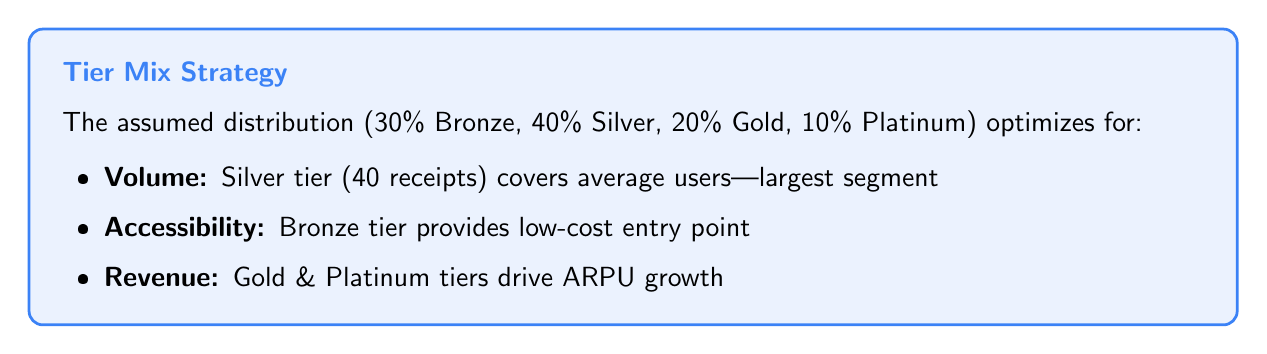
\begin{tikzpicture}
    \node[fill=infoblue!10, draw=infoblue, line width=1pt, rounded corners=5pt,
          inner sep=12pt, text width=14.5cm, align=left] {
        \textcolor{infoblue}{\textbf{Tier Mix Strategy}}\\[6pt]
        The assumed distribution (30\% Bronze, 40\% Silver, 20\% Gold, 10\% Platinum) optimizes for:
        \begin{itemize}[leftmargin=1.5em, itemsep=2pt]
            \item \textbf{Volume:} Silver tier (40 receipts) covers average users---largest segment
            \item \textbf{Accessibility:} Bronze tier provides low-cost entry point
            \item \textbf{Revenue:} Gold \& Platinum tiers drive ARPU growth
        \end{itemize}
    };
\end{tikzpicture}
\end{center}

\newpage

% ============================================================================
% API COST DEEP DIVE
% ============================================================================
\section*{\textcolor{miloprimary}{API Cost Deep Dive}}

\subsection*{\textcolor{milosecondary}{Veryfi OCR --- Primary Cost Driver (77\% of Variable Costs)}}

\begin{center}
\renewcommand{\arraystretch}{1.5}
\begin{tabular}{>{\raggedright\arraybackslash}p{4cm} >{\centering\arraybackslash}p{3.5cm} >{\centering\arraybackslash}p{3.5cm}}
\toprule
\rowcolor{warningorange!15}
\textbf{Volume Tier} & \textbf{Monthly Receipts} & \textbf{Price/Receipt} \\
\midrule
Starter & 0 -- 1,000 & \$0.10 \\
\rowcolor{lightbg}
Growth & 1,001 -- 10,000 & \$0.08 \\
Scale & 10,001 -- 100,000 & \$0.06 -- \$0.08 \\
\rowcolor{lightbg}
Enterprise & 100,000+ & \$0.04 -- \$0.06 (negotiated) \\
\bottomrule
\end{tabular}
\end{center}

\vspace{0.3cm}

\begin{center}
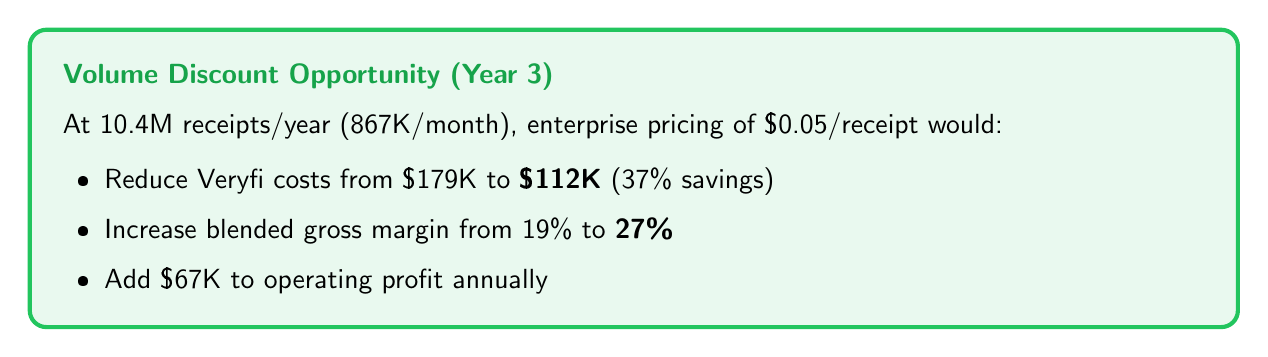
\begin{tikzpicture}
    \node[fill=successgreen!10, draw=successgreen, line width=1.5pt, rounded corners=6pt,
          inner sep=12pt, text width=14.5cm, align=left] {
        \textcolor{darkgreen}{\textbf{Volume Discount Opportunity (Year 3)}}\\[6pt]
        At 10.4M receipts/year (867K/month), enterprise pricing of \$0.05/receipt would:
        \begin{itemize}[leftmargin=1.5em, itemsep=2pt]
            \item Reduce Veryfi costs from \$179K to \textbf{\$112K} (37\% savings)
            \item Increase blended gross margin from 19\% to \textbf{27\%}
            \item Add \$67K to operating profit annually
        \end{itemize}
    };
\end{tikzpicture}
\end{center}

\vspace{0.5cm}

\subsection*{\textcolor{milosecondary}{Gemini 2.0 Flash --- AI Processing (3\% of Variable Costs)}}

\begin{center}
\renewcommand{\arraystretch}{1.4}
\begin{tabular}{>{\raggedright\arraybackslash}p{4cm} >{\centering\arraybackslash}p{2.5cm} >{\centering\arraybackslash}p{2.5cm} >{\centering\arraybackslash}p{2.5cm}}
\toprule
\rowcolor{miloprimary!15}
\textbf{Function} & \textbf{Input Tokens} & \textbf{Output Tokens} & \textbf{Cost/Call} \\
\midrule
Receipt Categorization & ~500 & ~300 & \$0.00017 \\
\rowcolor{lightbg}
AI Chat Message & ~2,000 & ~500 & \$0.00040 \\
Health Score Calculation & ~200 & ~100 & \$0.00006 \\
\bottomrule
\end{tabular}
\end{center}

\vspace{0.3cm}

\begin{center}

\begin{tikzpicture}
    \node[fill=lightbg, draw=freegray, line width=1pt, rounded corners=5pt,
          inner sep=10pt, text width=14.5cm, align=center] {
        \textcolor{freegray}{\textbf{Assessment:}} Gemini costs are \textbf{negligible} at <3\% of variable costs.\\
        Even a 200\% price increase would only impact margins by ~0.5\%.
    };
\end{tikzpicture}
\end{center}

\vspace{0.5cm}

\subsection*{\textcolor{milosecondary}{Payment Processing Costs}}

\begin{center}
\renewcommand{\arraystretch}{1.4}
\begin{tabular}{>{\raggedright\arraybackslash}p{5cm} >{\centering\arraybackslash}p{3cm} >{\centering\arraybackslash}p{5cm}}
\toprule
\rowcolor{miloprimary!15}
\textbf{Channel} & \textbf{Rate} & \textbf{Notes} \\
\midrule
Apple App Store (Year 1) & 15\% & Small Business Program (<\$1M) \\
\rowcolor{lightbg}
Apple App Store (Year 2+) & 15\% & Retained subscriber rate \\
Google Play Store & 15\% & Small Business Program \\
\rowcolor{lightbg}
Stripe (B2B Direct) & 2.9\% + \$0.30 & Enterprise/direct deals \\
\bottomrule
\end{tabular}
\end{center}

\newpage

% ============================================================================
% FIXED COSTS STRUCTURE
% ============================================================================
\section*{\textcolor{miloprimary}{Fixed Costs Structure}}

\subsection*{\textcolor{milosecondary}{Fixed Cost Projections (3-Year)}}

\begin{center}
\renewcommand{\arraystretch}{1.5}
\begin{tabular}{>{\raggedright\arraybackslash}p{4.5cm} >{\centering\arraybackslash}p{2.8cm} >{\centering\arraybackslash}p{2.8cm} >{\centering\arraybackslash}p{2.8cm}}
\toprule
\rowcolor{miloprimary!15}
\textbf{Category} & \textbf{Year 1} & \textbf{Year 2} & \textbf{Year 3} \\
\midrule
\textbf{Engineering \& Product} & \$100K & \$180K & \$300K \\
\rowcolor{lightbg}
\textbf{Sales \& Marketing} & \$75K & \$150K & \$200K \\
\textbf{B2B Sales Team} & \$25K & \$80K & \$120K \\
\rowcolor{lightbg}
\textbf{Legal \& Compliance (GDPR)} & \$40K & \$60K & \$75K \\
\textbf{Customer Support} & \$10K & \$25K & \$40K \\
\rowcolor{lightbg}
\textbf{Infrastructure (non-API)} & \$10K & \$15K & \$20K \\
\midrule
\rowcolor{miloprimary!15}
\textbf{Total Fixed Costs} & \textbf{\$260K} & \textbf{\$510K} & \textbf{\$755K} \\
\bottomrule
\end{tabular}
\end{center}

\vspace{0.5cm}

\subsection*{\textcolor{milosecondary}{Fixed Cost per User Analysis}}

\begin{center}
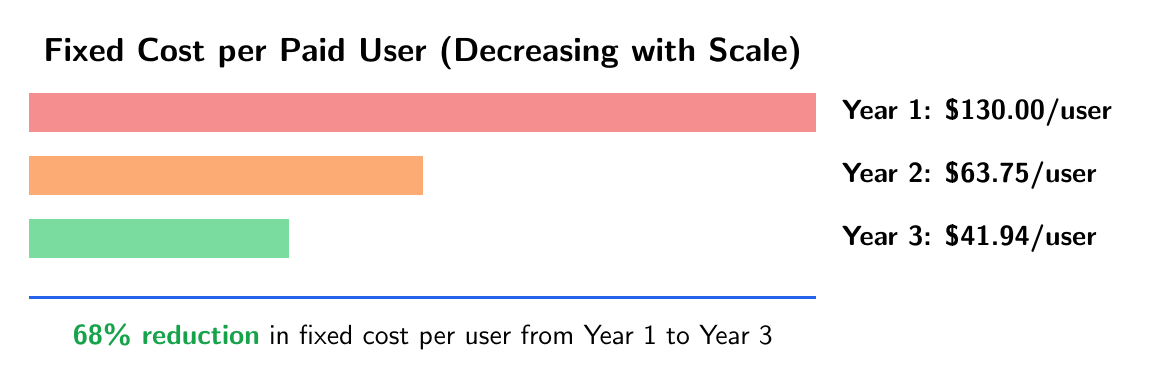
\begin{tikzpicture}
    % Title
    \node[align=center] at (0,3.8) {\textbf{\large Fixed Cost per Paid User (Decreasing with Scale)}};

    % Year 1 bar
    \fill[dangerred!60] (-5,2.8) rectangle (5,3.3);
    \node[right] at (5.2,3.05) {\textbf{Year 1: \$130.00/user}};

    % Year 2 bar
    \fill[warningorange!60] (-5,2) rectangle (0,2.5);
    \node[right] at (5.2,2.25) {\textbf{Year 2: \$63.75/user}};

    % Year 3 bar
    \fill[successgreen!60] (-5,1.2) rectangle (-1.7,1.7);
    \node[right] at (5.2,1.45) {\textbf{Year 3: \$41.94/user}};

    % Improvement note
    \draw[line width=1pt, miloprimary] (-5,0.7) -- (5,0.7);
    \node[align=center] at (0,0.2) {\textcolor{darkgreen}{\textbf{68\% reduction}} in fixed cost per user from Year 1 to Year 3};
\end{tikzpicture}
\end{center}

\vspace{0.5cm}

\begin{center}
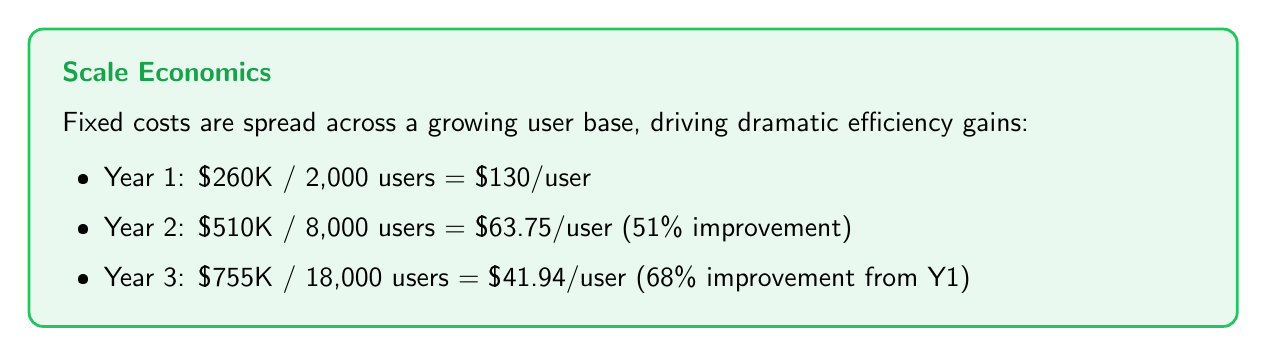
\begin{tikzpicture}
    \node[fill=successgreen!10, draw=successgreen, line width=1pt, rounded corners=5pt,
          inner sep=12pt, text width=14.5cm, align=left] {
        \textcolor{darkgreen}{\textbf{Scale Economics}}\\[6pt]
        Fixed costs are spread across a growing user base, driving dramatic efficiency gains:
        \begin{itemize}[leftmargin=1.5em, itemsep=2pt]
            \item Year 1: \$260K / 2,000 users = \$130/user
            \item Year 2: \$510K / 8,000 users = \$63.75/user (51\% improvement)
            \item Year 3: \$755K / 18,000 users = \$41.94/user (68\% improvement from Y1)
        \end{itemize}
    };
\end{tikzpicture}
\end{center}

\newpage

% ============================================================================
% PROFITABILITY ANALYSIS
% ============================================================================
\section*{\textcolor{miloprimary}{Profitability Analysis}}

\subsection*{\textcolor{milosecondary}{Revenue Model}}

\begin{center}
\renewcommand{\arraystretch}{1.5}
\begin{tabular}{>{\raggedright\arraybackslash}p{4cm} >{\centering\arraybackslash}p{3cm} >{\centering\arraybackslash}p{3cm} >{\centering\arraybackslash}p{3cm}}
\toprule
\rowcolor{miloprimary!15}
\textbf{Tier} & \textbf{Year 1 Revenue} & \textbf{Year 2 Revenue} & \textbf{Year 3 Revenue} \\
\midrule
\rowcolor{bronzecolor!8}
Bronze (\$2 $\times$ 30\%) & \$14K & \$58K & \$130K \\
\rowcolor{silvercolor!8}
Silver (\$4 $\times$ 40\%) & \$38K & \$154K & \$346K \\
\rowcolor{goldcolor!8}
Gold (\$6 $\times$ 20\%) & \$29K & \$115K & \$259K \\
\rowcolor{platinumcolor!8}
Platinum (\$10 $\times$ 10\%) & \$24K & \$96K & \$216K \\
\midrule
\rowcolor{lightbg}
\textbf{B2B Revenue (15\%)} & \$39K & \$297K & \$849K \\
\midrule
\rowcolor{successgreen!15}
\textbf{Total Revenue} & \textbf{\$144K} & \textbf{\$720K} & \textbf{\$1.8M} \\
\bottomrule
\end{tabular}
\end{center}

\vspace{0.5cm}

\subsection*{\textcolor{milosecondary}{Profit \& Loss Summary}}

\begin{center}
\renewcommand{\arraystretch}{1.6}
\begin{tabular}{>{\raggedright\arraybackslash}p{5cm} >{\centering\arraybackslash}p{2.8cm} >{\centering\arraybackslash}p{2.8cm} >{\centering\arraybackslash}p{2.8cm}}
\toprule
\rowcolor{miloprimary!15}
\textbf{Metric} & \textbf{Year 1} & \textbf{Year 2} & \textbf{Year 3} \\
\midrule
\textbf{Revenue} & \$144K & \$720K & \$1,800K \\
\rowcolor{lightbg}
Variable Costs & (\$36K) & (\$116K) & (\$232K) \\
\textbf{Gross Profit} & \$108K & \$604K & \$1,568K \\
\rowcolor{successgreen!10}
\textbf{Gross Margin} & \textbf{75\%} & \textbf{84\%} & \textbf{87\%} \\
\midrule
\rowcolor{lightbg}
Fixed Costs & (\$260K) & (\$510K) & (\$755K) \\
\rowcolor{dangerred!10}
\textbf{Operating Profit/(Loss)} & \textbf{(\$152K)} & \textbf{\$94K} & \textbf{\$813K} \\
\textbf{Operating Margin} & -106\% & \textbf{13\%} & \textbf{45\%} \\
\bottomrule
\end{tabular}
\end{center}

\vspace{0.5cm}

\begin{center}
\alertbox{successgreen}{Strong Path to Profitability}{
\begin{itemize}[leftmargin=1.5em, itemsep=4pt]
    \item \textbf{Year 1:} Investment phase with \$152K operating loss (manageable with seed funding)
    \item \textbf{Year 2:} Break-even achieved with \$94K operating profit (13\% margin)
    \item \textbf{Year 3:} Strong profitability with \$813K operating profit (45\% margin)
    \item \textbf{Gross margins} improve from 75\% to 87\% as payment processing efficiencies kick in
\end{itemize}
}
\end{center}

\newpage

% ============================================================================
% UNIT ECONOMICS
% ============================================================================
\section*{\textcolor{miloprimary}{Unit Economics Analysis}}

\subsection*{\textcolor{milosecondary}{Per-User Economics}}

\begin{center}
\renewcommand{\arraystretch}{1.6}
\begin{tabular}{>{\raggedright\arraybackslash}p{5cm} >{\centering\arraybackslash}p{3cm} >{\centering\arraybackslash}p{3cm} >{\centering\arraybackslash}p{3cm}}
\toprule
\rowcolor{miloprimary!15}
\textbf{Metric} & \textbf{Year 1} & \textbf{Year 2} & \textbf{Year 3} \\
\midrule
Paid Users & 2,000 & 8,000 & 18,000 \\
\rowcolor{lightbg}
ARPU (Monthly) & \$6.00 & \$6.25 & \$6.48 \\
ARPU (Annual) & \$72.00 & \$75.00 & \$77.78 \\
\midrule
\rowcolor{lightbg}
Variable Cost/User (Annual) & \$18.00 & \$14.50 & \$12.89 \\
Fixed Cost/User (Annual) & \$130.00 & \$63.75 & \$41.94 \\
\rowcolor{warningorange!10}
\textbf{Total Cost/User (Annual)} & \textbf{\$148.00} & \textbf{\$78.25} & \textbf{\$54.83} \\
\midrule
\rowcolor{successgreen!10}
\textbf{Profit/(Loss) per User} & \textbf{(\$76.00)} & \textbf{(\$3.25)} & \textbf{\$22.95} \\
\bottomrule
\end{tabular}
\end{center}

\vspace{0.5cm}

\subsection*{\textcolor{milosecondary}{Customer Lifetime Value (LTV)}}

\begin{center}
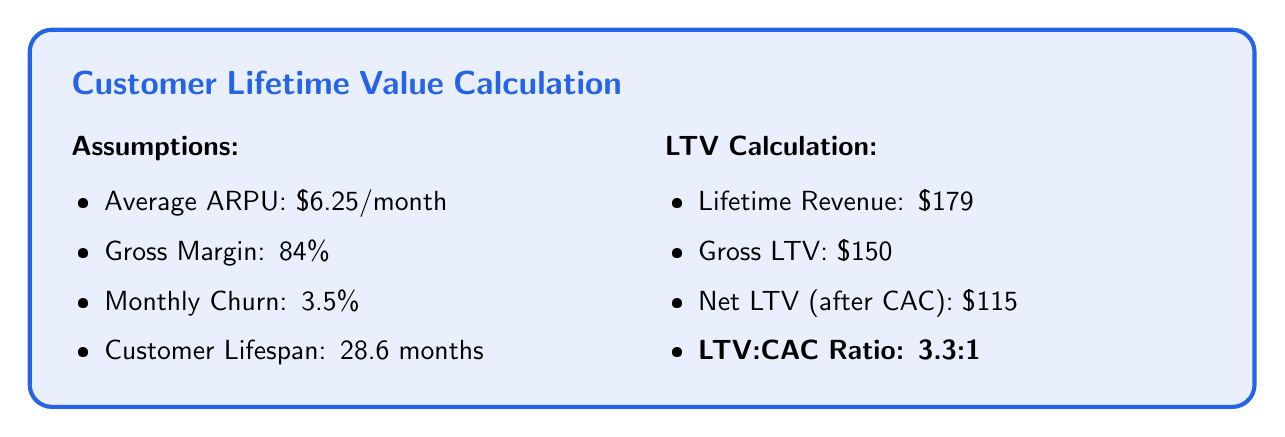
\begin{tikzpicture}
    \node[fill=miloprimary!10, draw=miloprimary, line width=1.5pt, rounded corners=8pt,
          inner sep=15pt, text width=14.5cm, align=left] {
        \textcolor{miloprimary}{\textbf{\large Customer Lifetime Value Calculation}}\\[10pt]
        \begin{minipage}[t]{0.48\textwidth}
            \textbf{Assumptions:}
            \begin{itemize}[leftmargin=1.2em, itemsep=2pt]
                \item Average ARPU: \$6.25/month
                \item Gross Margin: 84\%
                \item Monthly Churn: 3.5\%
                \item Customer Lifespan: 28.6 months
            \end{itemize}
        \end{minipage}
        \hfill
        \begin{minipage}[t]{0.48\textwidth}
            \textbf{LTV Calculation:}
            \begin{itemize}[leftmargin=1.2em, itemsep=2pt]
                \item Lifetime Revenue: \$179
                \item Gross LTV: \$150
                \item Net LTV (after CAC): \$115
                \item \textbf{LTV:CAC Ratio: 3.3:1}
            \end{itemize}
        \end{minipage}
    };
\end{tikzpicture}
\end{center}

\vspace{0.5cm}

\begin{center}
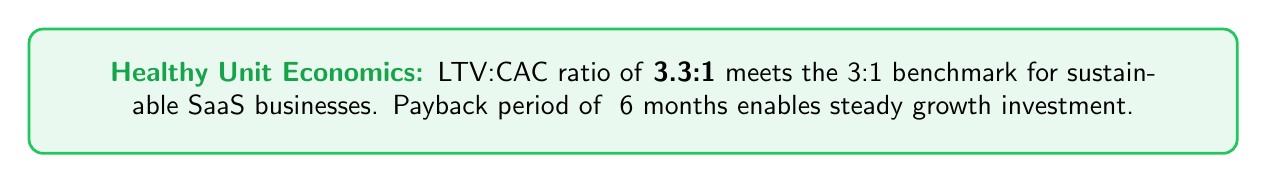
\begin{tikzpicture}
    \node[fill=successgreen!10, draw=successgreen, line width=1pt, rounded corners=5pt,
          inner sep=12pt, text width=14.5cm, align=center] {
        \textcolor{darkgreen}{\textbf{Healthy Unit Economics:}} LTV:CAC ratio of \textbf{3.3:1} meets the 3:1 benchmark for sustainable SaaS businesses. Payback period of ~6 months enables steady growth investment.
    };
\end{tikzpicture}
\end{center}

\newpage

% ============================================================================
% SENSITIVITY ANALYSIS
% ============================================================================
\section*{\textcolor{miloprimary}{Risk \& Sensitivity Analysis}}

\subsection*{\textcolor{milosecondary}{Key Variable Sensitivity (Year 3)}}

\begin{center}
\renewcommand{\arraystretch}{1.5}
\begin{tabular}{>{\raggedright\arraybackslash}p{4cm} >{\centering\arraybackslash}p{2.5cm} >{\centering\arraybackslash}p{2.5cm} >{\centering\arraybackslash}p{2.5cm} >{\centering\arraybackslash}p{2cm}}
\toprule
\rowcolor{miloprimary!15}
\textbf{Variable} & \textbf{-20\%} & \textbf{Base Case} & \textbf{+20\%} & \textbf{Risk} \\
\midrule
Veryfi OCR Cost & +\$36K profit & \$813K & -\$36K profit & \cellcolor{warningorange!20}Medium \\
\rowcolor{lightbg}
User Growth & \$570K profit & \$813K & \$1,056K profit & \cellcolor{warningorange!20}Medium \\
ARPU & \$453K profit & \$813K & \$1,173K profit & \cellcolor{warningorange!20}Medium \\
\rowcolor{lightbg}
Engineering Costs & +\$60K profit & \$813K & -\$60K profit & \cellcolor{successgreen!20}Low \\
\bottomrule
\end{tabular}
\end{center}

\vspace{0.5cm}

\subsection*{\textcolor{milosecondary}{Scenario Analysis}}

\begin{center}
\renewcommand{\arraystretch}{1.5}
\begin{tabular}{>{\raggedright\arraybackslash}p{4cm} >{\centering\arraybackslash}p{2.5cm} >{\centering\arraybackslash}p{2.5cm} >{\centering\arraybackslash}p{2.5cm} >{\centering\arraybackslash}p{2.5cm}}
\toprule
\rowcolor{miloprimary!15}
\textbf{Scenario} & \textbf{Year 1} & \textbf{Year 2} & \textbf{Year 3} & \textbf{Probability} \\
\midrule
\rowcolor{dangerred!10}
\textbf{Bear Case} & (\$190K) & (\$50K) & \$350K & 20\% \\
\rowcolor{lightbg}
\textbf{Base Case} & (\$152K) & \$94K & \$813K & 60\% \\
\rowcolor{successgreen!10}
\textbf{Bull Case} & (\$100K) & \$250K & \$1,300K & 20\% \\
\bottomrule
\end{tabular}
\end{center}

\vspace{0.5cm}

\subsection*{\textcolor{milosecondary}{Risk Mitigation Strategies}}

\begin{center}
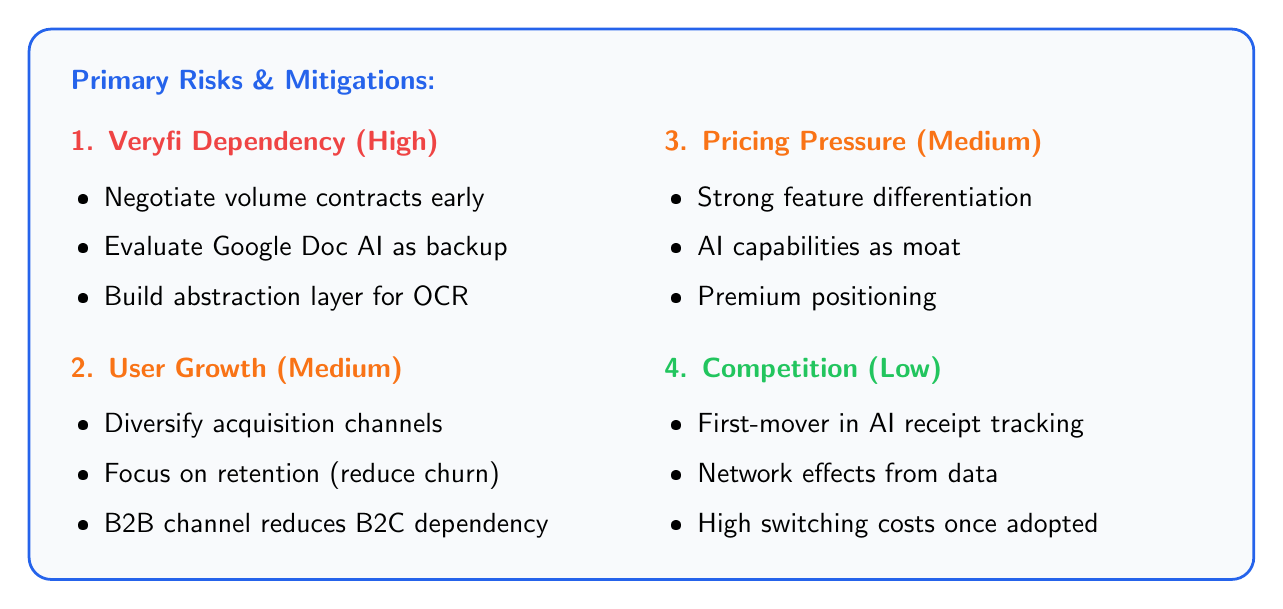
\begin{tikzpicture}
    \node[fill=lightbg, draw=miloprimary, line width=1pt, rounded corners=8pt,
          inner sep=15pt, text width=14.5cm, align=left] {
        \textcolor{miloprimary}{\textbf{Primary Risks \& Mitigations:}}\\[10pt]
        \begin{minipage}[t]{0.48\textwidth}
            \textcolor{dangerred}{\textbf{1. Veryfi Dependency (High)}}
            \begin{itemize}[leftmargin=1.2em, itemsep=2pt]
                \item Negotiate volume contracts early
                \item Evaluate Google Doc AI as backup
                \item Build abstraction layer for OCR
            \end{itemize}
            \vspace{6pt}
            \textcolor{warningorange}{\textbf{2. User Growth (Medium)}}
            \begin{itemize}[leftmargin=1.2em, itemsep=2pt]
                \item Diversify acquisition channels
                \item Focus on retention (reduce churn)
                \item B2B channel reduces B2C dependency
            \end{itemize}
        \end{minipage}
        \hfill
        \begin{minipage}[t]{0.48\textwidth}
            \textcolor{warningorange}{\textbf{3. Pricing Pressure (Medium)}}
            \begin{itemize}[leftmargin=1.2em, itemsep=2pt]
                \item Strong feature differentiation
                \item AI capabilities as moat
                \item Premium positioning
            \end{itemize}
            \vspace{6pt}
            \textcolor{successgreen}{\textbf{4. Competition (Low)}}
            \begin{itemize}[leftmargin=1.2em, itemsep=2pt]
                \item First-mover in AI receipt tracking
                \item Network effects from data
                \item High switching costs once adopted
            \end{itemize}
        \end{minipage}
    };
\end{tikzpicture}
\end{center}

\newpage

% ============================================================================
% CONCLUSION
% ============================================================================
\section*{\textcolor{miloprimary}{Conclusion \& Recommendations}}

\begin{center}
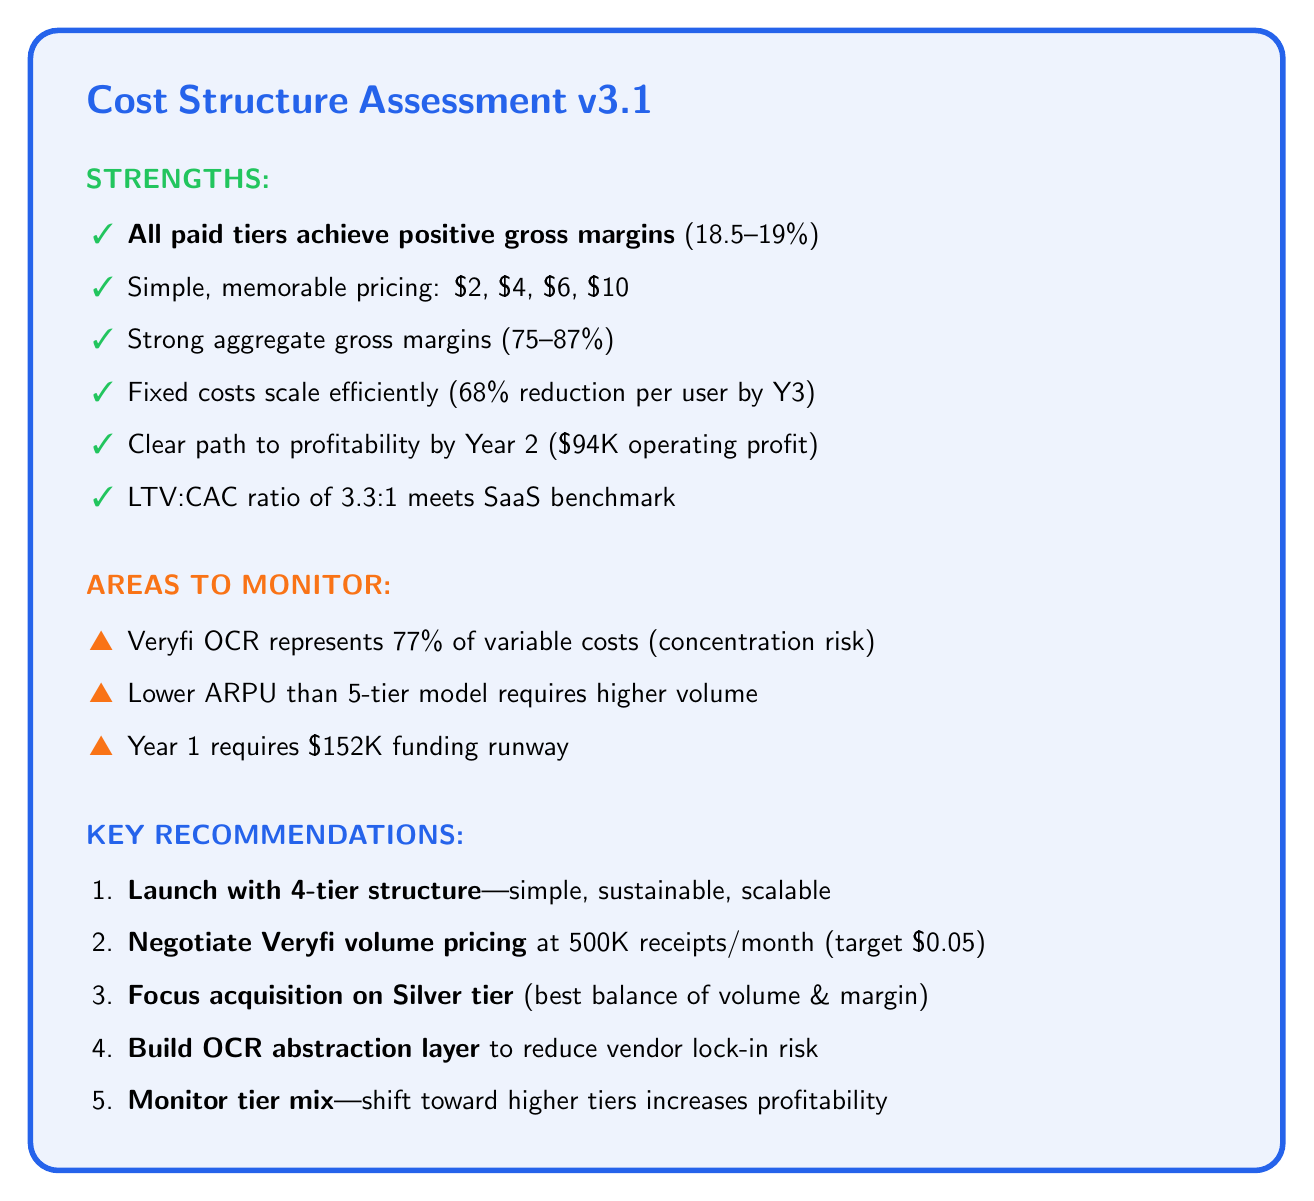
\begin{tikzpicture}
    \node[fill=miloprimary!8, draw=miloprimary, line width=2pt, rounded corners=10pt,
          inner sep=20pt, text width=14.5cm, align=left] {
        {\Large\textcolor{miloprimary}{\textbf{Cost Structure Assessment v3.1}}}\\[15pt]

        \textcolor{successgreen}{\textbf{STRENGTHS:}}
        \begin{itemize}[leftmargin=1.5em, itemsep=3pt]
            \item[\cmark] \textbf{All paid tiers achieve positive gross margins} (18.5--19\%)
            \item[\cmark] Simple, memorable pricing: \$2, \$4, \$6, \$10
            \item[\cmark] Strong aggregate gross margins (75--87\%)
            \item[\cmark] Fixed costs scale efficiently (68\% reduction per user by Y3)
            \item[\cmark] Clear path to profitability by Year 2 (\$94K operating profit)
            \item[\cmark] LTV:CAC ratio of 3.3:1 meets SaaS benchmark
        \end{itemize}

        \vspace{12pt}
        \textcolor{warningorange}{\textbf{AREAS TO MONITOR:}}
        \begin{itemize}[leftmargin=1.5em, itemsep=3pt]
            \item[\wmark] Veryfi OCR represents 77\% of variable costs (concentration risk)
            \item[\wmark] Lower ARPU than 5-tier model requires higher volume
            \item[\wmark] Year 1 requires \$152K funding runway
        \end{itemize}

        \vspace{12pt}
        \textcolor{miloprimary}{\textbf{KEY RECOMMENDATIONS:}}
        \begin{itemize}[leftmargin=1.5em, itemsep=3pt]
            \item[1.] \textbf{Launch with 4-tier structure}---simple, sustainable, scalable
            \item[2.] \textbf{Negotiate Veryfi volume pricing} at 500K receipts/month (target \$0.05)
            \item[3.] \textbf{Focus acquisition on Silver tier} (best balance of volume \& margin)
            \item[4.] \textbf{Build OCR abstraction layer} to reduce vendor lock-in risk
            \item[5.] \textbf{Monitor tier mix}---shift toward higher tiers increases profitability
        \end{itemize}
    };
\end{tikzpicture}
\end{center}

\vspace{0.8cm}

% Summary Statistics
\begin{center}
    \statbox{successgreen}{Gross Margin}{75--87\%}
    \hspace{0.3cm}
    \statbox{miloprimary}{Break-even}{Year 2}
    \hspace{0.3cm}
    \statbox{goldcolor}{Y3 Revenue}{\$1.8M}
    \hspace{0.3cm}
    \statbox{darkgreen}{Y3 Profit}{\$813K}
\end{center}

\vspace{1cm}

% Footer
\begin{center}
    \textcolor{freegray}{\rule{14cm}{0.5pt}}\\[0.4cm]
    \textcolor{freegray}{\small DeepmAInd B.V. | Confidential | Version 3.1 | January 2026}\\[0.2cm]
    \textcolor{freegray}{\scriptsize Data sources: Federal Reserve Diary of Consumer Payment Choice (2024), Veryfi API Pricing, Google Gemini Pricing}
\end{center}

\end{document}
